\section{Implementazione}
In questa sezione vengono descritte le principali classi e interfacce implementate, organizzate nei rispettivi package in base al loro ruolo all'interno del sistema.

\subsection{Domain Model}
Il Domain Model, mostrato in Figura~\ref{fig:domain_model}, rappresenta l'insieme delle entità fondamentali del dominio applicativo e le relazioni tra di esse. 
Ogni classe modella un concetto reale presente nel sistema di gestione della biblioteca.
\begin{figure}[H]
    \centering
    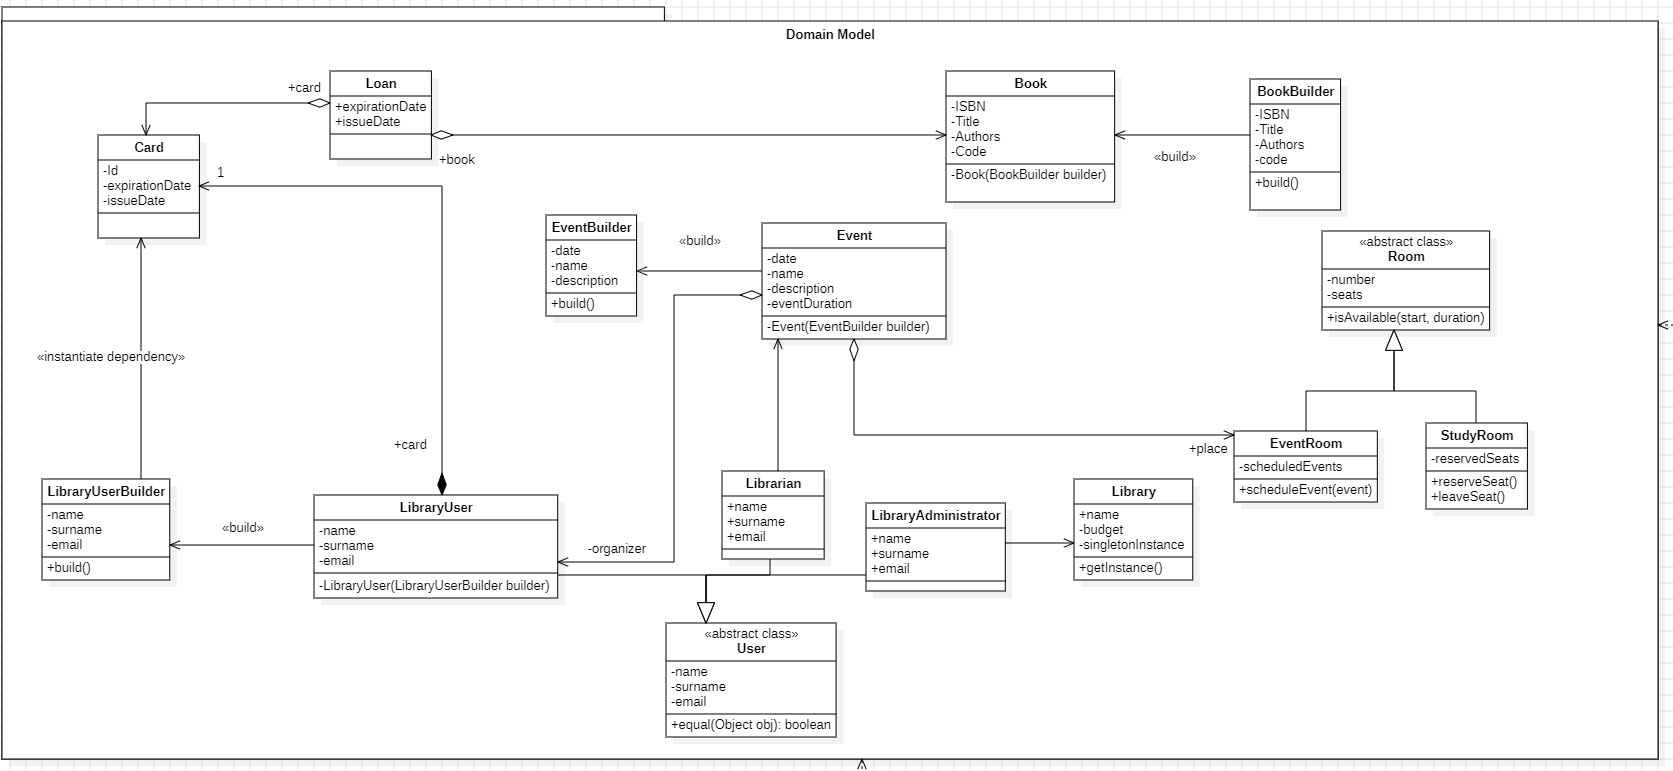
\includegraphics[width=\linewidth]{images/class diagram/domain_model.png}
    \caption{Domain Model del sistema}
    \label{fig:domain_model}
\end{figure}

    \subsubsection{Library}
    Questa classe rappresenta la biblioteca. È caratterizzata da un nome ed un budget che ha a disposizione.\\
    Per l'istanza di una Library viene utilizzato il design pattern del \textbf{singleton}, in modo tale da avere un unica istanza in tutto il sistema.
    
    \subsubsection{Book}
    Questa classe rappresenta un libro.\\
    Questo può essere aggiunto o rimosso dal catalogo di tutti i libri della biblioteca da parte dell'amministratore della biblioteca. Se presente nel catalogo, può essere preso in prestito da un utente ed è identificato tramite ISBN, titolo e codice. Inoltre su questo è riportato anche il nome degli autori.\\
    Per la creazione di un oggetto Book viene usato il \textbf{BookBuilder}, che implementa il design pattern del \textbf{builder}.\\

    \subsubsection{Loan}
    Questa classe rappresenta un prestito di un libro da parte di un utente.\\

    \subsubsection{User}
    Questa classe rappresenta un utente astratto, caratterizzato da nome, cognome ed email. La classe appunto è definita come astratta.\\

     \subsubsection{LibraryUser}
    Questa classe rappresenta un utente che può usufruire i servizi messi a disposizione dalla biblioteca, come il prestito di libri, l'iscrizione ad eventi o la prenotazione posti nelle aule studio.\\
    La creazione degli oggetti avviene tramite il design pattern \textbf{Builder}.
    
    \subsubsection{Librarian}
    Questa classe rappresenta un bibliotecario, un utente con permessi aggiuntivi, che lavora all'interno della biblioteca. Può gestire gli eventi, creare/rinnovare tessere della biblioteca e monitorare i prestiti.\\
    
    \subsubsection{LibraryAdministrator}
    Questa classe rappresenta l'amministratore della biblioteca.\\
    Oltre alla gestione del catalogo libri, è anche responsabile dei fondi della biblioteca.
    
    \subsubsection{Card}
    Questa classe rappresenta una tessera della biblioteca associata a un utente.\\
    La tessera consente l'accesso ai servizi della biblioteca, come il prestito di libri e la prenotazione di risorse ed è identificata tramite id, data di emissione e scadenza della carta.\\
    
    \subsubsection{Event}
    Questa classe rappresenta un evento organizzato dalla biblioteca.\\
    È identificato tramite un id univoco e caratterizzato da nome, descrizione, data, durata e luogo.\\
    La creazione degli oggetti avviene tramite l'\textbf{EventBuilder}, che implementa il design pattern \textbf{Builder}.\\

    \subsubsection{Room}
    Questa classe rappresenta una stanza generica della biblioteca.\\
    È identificata tramite un numero, la sua capacità e un attributo che indica se si tratta di un aula studio.\\
    
    \subsubsection{EventRoom}
    Questa classe rappresenta una stanza che può essere adibita allo svolgimento di eventi.\\
    
    \subsubsection{StudyRoom}
    Questa classe rappresenta una stanza dedicata esclusivamente per lo studio.\\
    


\subsection{Business Logic}
La Business Logic, mostrata in Figura~\ref{fig:business_logic}, contiene tutte le classi responsabili della gestione delle funzionalità del sistema e dell'interazione tra le diverse entità del Domain Model.
\begin{figure}[H]
    \centering
    
\includegraphics[width=\linewidth]{images/class diagram/business_logic.png}
    \caption{Business Logic del sistema}
    \label{fig:business_logic}
\end{figure}

    \subsubsection{AuthService e ConcreteAuthService}
    L'\texttt{AuthService} è un'interfaccia che dichiara i principali metodi di autenticazione: \textbf{login, logout, register e resetPassword,}.\\
    Questi vengono implementati in \texttt{ConcreteAuthService}. In particolare, il metodo \textbf{login} restituisce un tipo di utente diverso in base al ruolo dell'utente autenticato.\\
    La gestione della sessione di un utente, è realizzato tramite il metodo \textbf{isLogged}, che verifica se un utente è autenticato o meno.\\

    \subsubsection{role}
    Il \texttt{role} è un \textbf{enum} che identifica i possibili ruoli degli utenti del sistema: \textbf{LibraryUser, Librarian e LibraryAdministrator}.\\

    \subsubsection{ControllerInterface}
    La \texttt{ControllerInterface} è un'interfaccia di supporto, che dichiara il metodo \textbf{createController}, il quale restituisce un oggetto di tipo \texttt{ControllerInterface}.\\
    Questa interfaccia implementa il design pattern \textbf{Factory}, consentendo la creazione dei diversi controller in base al tipo di utente.

    \subsubsection{ControllerFactory}
    La \texttt{ControllerFactory} è un'interfaccia che dichiara il metodo \textbf{createController}, il quale restituisce un oggetto di tipo \texttt{ControllerInterface}.\\
    Questa interfaccia implementa il design pattern \textbf{Factory}, consentendo la creazione dei diversi controller in base al tipo di utente.

    \subsubsection{LibraryUserControllerFactory}
    Questa classe implementa l'interfaccia \texttt{ControllerFactory} e sovrascrive il metodo \textbf{createController}, restituendo un'istanza di \texttt{LibraryUserController}.

    \subsubsection{LibraryUserController}
    La classe \texttt{LibraryUserController} definisce un interfaccia per gli utenti della biblioteca che come anticipato possono:
    \begin{itemize}
        \item richiedere in prestito un libro con \textbf{requestLoan}, se l'utente possiede una carta non scaduta e se il libro è disponibile nel catalogo. 
        \item richiedere una tessera della biblioteca con \textbf{requestCard}, se l'utente non nè possiede già una.
        \item prenotare un posto in un aula studio con \textbf{reserveSeatStudyRoom}, se l'utente non ha già effettuato una prenotazione e se la stanza non è piena.
        \item lasciare un posto in un aula studio con \textbf{leaveSeatStudyRoom}.
        \item prenotare un posto ad un evento con \textbf{eventBooking}.
        \item cancellare una prenotazione ad un evento con \textbf{cancelEventBooking}.
    \end{itemize}

    \subsubsection{LibrarianControllerFactory}
    Questa classe implementa l'interfaccia \texttt{ControllerFactory} e sovrascrive il metodo \textbf{createController}, restituendo un'istanza di \texttt{LibrarianController}.

    \subsubsection{LibrarianController}
    La classe \texttt{LibrarianController} definisce invece tutte le operazioni per i bibliotecari, che sono:
    \begin{itemize}
        \item creare o rinnovare una tessera con \textbf{createCard}.
        \item creare un evento con \textbf{createEvent}.
        \item cancellare un evento con \textbf{cancelEvent}.
        \item modificare un evento con \textbf{modifyEvent}.
        \item registrare un prestito con \textbf{registerLoan}.
        \item rinnovare un prestito con \textbf{grantLoan}.
        \item terminare un prestito con \textbf{endLoan}.
    \end{itemize}

    \subsubsection{LibraryAdministratorControllerFactory}
    Questa classe implementa l'interfaccia \texttt{ControllerFactory} e sovrascrive il metodo \textbf{createController}, restituendo un'istanza di \texttt{LibraryAdministratorController}.

    \subsubsection{LibraryAdministratorController}
    La classe \texttt{LibraryAdministratorController} infine definisce tutte le operazioni disponibili per l'amministratore della biblioteca, che sono:
    \begin{itemize}
        \item aumentare il budget della biblioteca con \textbf{increaseBudget}, il quale non può essere negativo.
        \item aggiungere un libro al catalogo con \textbf{addBookToCatalogue}.
        \item rimuovere un libro dal catalogo con \textbf{removeBookFromCatalogue}.
        \item aggiornare un libro nel catalogo con \textbf{updateBookInCatalogue}.
    \end{itemize}

\subsection{ORM}